\section{\texorpdfstring{Non-uniform computation}{Non-uniform computation}}
\vspace{5mm}
\large
% 7th lecture

\begin{definition}[Uniform computation]
	Uniform models of computation - single algorithm for all inputs. (DTM, NTM, RAM ...)
\end{definition}

\begin{definition}[Non-uniform computation]
	Algorithm may vary for different input lengths.
	However, inputs of the same lengths are handled by the same algorithm.

	For example Boolean circuits.
\end{definition}

\begin{definition}[Boolean circuit]
	Boolean circuit with $n$ inputs (and single output) is an acyclic directed graph with $n$ source virtices.
	Source vertex has $deg_{in}(s) = 0$.
	And single sink vertex $deg_{out}(t) = 0$.

	Source vertices represents the inputs, sink - output.
	All other vertices are gates (NOT, AND, OR).

	AND, OR gates have 2 inputs (in degree).
	NOT has only 1 input.

	Size of the circuit is \# of vertices.
\end{definition}

\begin{note}
	Because of the selected elementary gates, number of edges is bounded by $2n$.
\end{note}

\begin{example}[XOR gate]
	$x_1 XOR x_2$ as a DNF formula:
	\[ (x_1 \land \neg x_2) \lor (\neg x_1 \land x_2) \]

	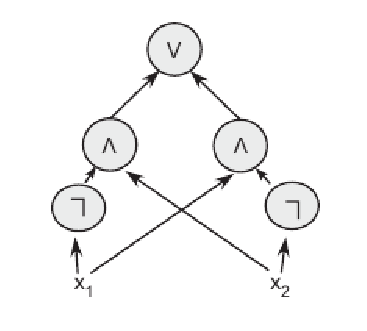
\includegraphics[scale=0.4]{xor_0.eps}

	Source ~\cite{arora2009computational}.

	Or CNF
	\[ (x_1 \lor x_2) \land (\neg x_1 \lor \neg x_2) \]
\end{example}

\begin{example}
	\[ (x_1 \lor x_2 \lor x_3) \land (x_1 \lor x_2 \lor x_4) \land (x_1 \lor x_2 \lor x_5) \]
	The gate will be the following:

	%lecture 7 25:00
	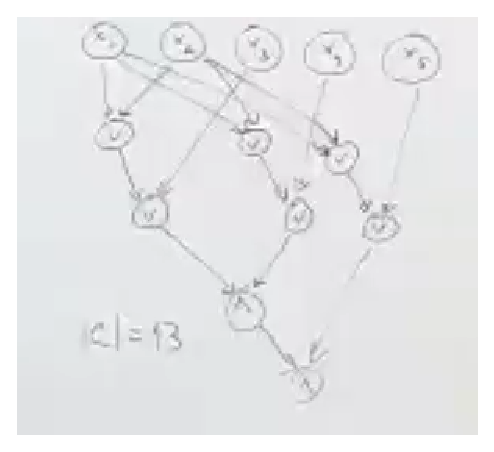
\includegraphics[scale=0.4]{gate_0.eps}

	Size of the gate is $|C| = 13$.

	However, if we change the definition and allow multiple outputs, size is $|C| = 11$.
	%lecture 7 25:00
	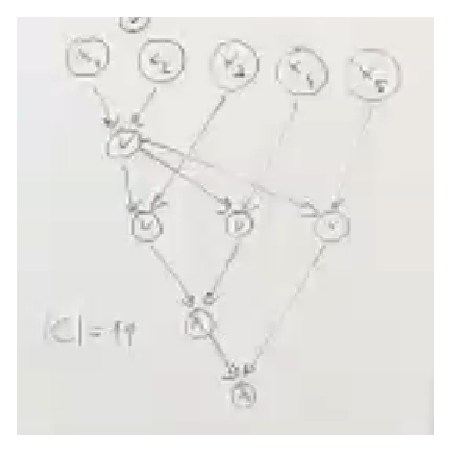
\includegraphics[scale=0.4]{gate_1.eps}
\end{example}

\begin{observation}
	If we allow gates with $k$ inputs or outputs, the equivalent binary circuit will have $(k - 1)$ gates.
	Depth of the tree can be optimized by balancing.

	%lecture 7 26:29
	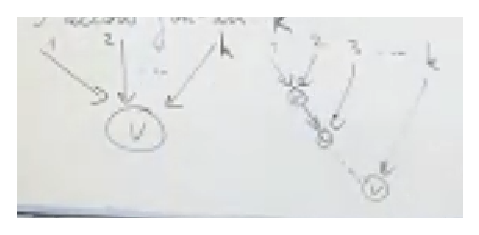
\includegraphics[scale=0.4]{gate_k.eps}
\end{observation}

\begin{note}
	Having gates with unlimited inputs can result in an exponential blowup.
\end{note}

Q: do we restrict the gates to binary? A: no, but we allow only finite?

\begin{note}
	Circuit with input of size $n$ can be viewed as an device that recognizes Language of binary words of length $n$.

	A sequence $\{C_n\}$ of circuits of various length is a device that recognizes some Language.
	Enormous switch by $n$.
\end{note}

\begin{notation}
	For circuit $C$ and input vector $x: C(x)$ is a value of the output gate.
\end{notation}

\begin{definition}[Family of circuits]
	Let $T$ be a function. A family of circuits of size $T(n)$ is a sequence of circuits $\{C_n\}_{n \in \N}$.
	Where
	\[ \forall n \in \N: C_n\ \text{has n inputs}\ \& |C_n| \leq T(n) \]

	Language $L$ is in class SIZE$(T(n))$ is there exists a family of circuits $\{C_n\}$ of size $T(n)$ such that
	\[ \forall x \in L \iff C_n(x) = 1 \]
\end{definition}

Q: $T$ is a boolean function?

\begin{example}
	\[ L = \{ 1^n |\ n \in \N \} \]
	Then $L \in $ SIZE$(\bigO(n))$.

	The circuit is a conjunction of all inputs.
\end{example}

\begin{example}
	\[ L = \{ (i, j, i + j) |\ i, j \in \N \} \]
	Then $L \in $ SIZE$(\bigO(n))$.

	The circuit performs binary addition of $i$ and $j$, then compare with $i + j$.
	Binary addition can be done by circuit of linear size.
\end{example}

\begin{definition}[$\Ppoly$ class]
	\[ \Ppoly = \bigcup^{\infty} SIZE (n^i) \]
	Class of languages recognizable by families of circuits of polynomial size.
\end{definition}

\begin{reminder}[Oblivious DTM]\label{obliv_dtm}
	IF $L$ is recognizable by DTM M in time $p(n)$ then it is also recognizable by DTM $M_1$ with single work tape with time complexity $p^2(n)$.
	Moreover, the positions of the heads of $M_1$ depend only on \# of steps that $M$ performed and NOT on the input.
\end{reminder}

\begin{theorem}[$\TP \subseteq \Ppoly$]\label{tp_ppoly}
	$\TP \subseteq \Ppoly$.
\end{theorem}
\begin{proof}
	Idea: for fixed input length $n$ TM can be simulated by polynomial size circuit.
	The only problem is to get the symbol from work/input tape without storing the whole tape.
	Which is solved by the previous configuration with current symbol.

	Let $L \in \TP$ be arbitrary. WLOG there is an oblivious DTM M \cref{obliv_dtm} such that $L = L(M)$.
	$M$ works in time $T(n)$, where $T$ is a polynomial.
	WLOG $T(n)$ is the exact time $M$ needs for computation.
	We can choose $T(n)$ by trying different polynomials in parallel with $M$ using the fact, that polynomials are \emph{time constructible}.

	Knowing that TM did exactly $T(n)$ steps tells us that there were $T(n)$ displays (state, input symbol, work tape symbol).

	Let $|x| = n$ be input, let
	\[ d_1, d_2, \ldots, d_{T(n)} \]
	be binary string encoding displays during the computation of $M$ on $x$.

	% todo not sure about this argument, lecture 7 01:20:00
	Since $M$ is \emph{oblivious}, the position of the head $i$ uniquely defines the position $i_v, i_p$.
	Because the position of the head is uniquely determined by the \# of steps.

	$i_v, i_p$ are the display indexes the last time the input head was in the same position and the work head was in the same position as in $d_i$.
	The gates representing the displays $d_{i_v}$ and $d_{i_p}$ are the inputs to the gate $C_i$.
	It can also happen, that next symbol under the head has not been seen during the computation yet.
	For such case, we add one more input $x_j$ - input bit.

	Similarly, $i_p$ should not be defined.
	However, we assume that work tape is blank before the computation and symbol is also blank.

	We should add one more gate that check whether TM finished in accepting state.
	Outputs 1 if was in accepting state and 0 o/w.

	Complexity: $|C_i| = \bigO(1) \Rightarrow |C| = \bigO(T(n))$.
\end{proof}

\begin{corollary}\label{tp_ppoly_cor}
	The family of circuits $\{C_n\}$ from previous theorem not only exists but also can be efficiently constructed.
	% todo missing word in place of ... lecture 7 01:29:50
	Meaning there exists DTM M which on the input $1^n$ (only marks the length) outputs a ... of $C_n$.
	Moreover M works in polynomial time and Log space.

	The only non-trivial thing in circuit construction is to compute indexes $i_v, i_p$ from $i$ and $n$.
	M outputs the circuit $C_i$ in $\bigO(\log n)$ time and space.

	Space is reused therefore total space complexity is also $\bigO(\log n)$.
	However, having $T(n)$ gates time complexity is $\bigO(T(n) * \log n)$ which is polynomial.
\end{corollary}

\begin{note}[$\TP \nsupseteq \Ppoly$]
	$\TP \supseteq \Ppoly$ is not true since every unary language
	\[ L \subseteq \{ 1^n |\ n \in \N \} \]
	is in $\Ppoly$.

	If $1^n \in L \Rightarrow C_n$ is a tree of $\land$.
	Otherwise, $C_n$ outputs 0.

	On the other side
	\[ UHALT = \{ 1^n |\ n\ \text{is a Godel number of}\ \langle M, x \rangle: M(x) \downarrow \} \]
	is not in $\TP$ as it is a variant of Halting problem which is undecidable.

	Q: how can boolean circuit recognize UHALT? How to detect that that TM halts in this case?
\end{note}

\begin{definition}[$\TP$-uniform family circuits]
	A family of circuits $\{C_n\}$ is $\TP$-uniform if there exists DTM M which on input $1^n$ outputs the description of $\{C_n\}$ and works in polynomial time.
\end{definition}

\begin{theorem}
	$L$ is accepted by $\TP$-uniform family of circuits $\iff L \in \TP$.
\end{theorem}
\begin{proof}
	"$\Rightarrow$". For an input $x$ DTM M will simulate DTM $M_g$ which outputs $C_n$ on $1^n$, guaranteed by uniformity.
	Then $M$ simulates $C_n$ on $x$.
	\[ x \in L(M) \iff C_n(x) = 1 \]

	"$\Leftarrow$". Follows from the corollary \cref{tp_ppoly_cor}.
\end{proof}

\begin{definition}[Log Space uniform family circuits]
	A family of circuits $\{C_n\}$ is $\TP$-uniform if there exists DTM M which on input $1^n$ outputs the description of $\{C_n\}$ and works in Log space.
\end{definition}

\begin{theorem}
	$L$ is accepted by Log Space uniform family of circuits $\iff L \in \TP$.
\end{theorem}
\begin{proof}
	"$\Rightarrow$". For an input $x$ DTM M will simulate DTM $M_g$ which outputs $C_n$ on $1^n$, guaranteed by uniformity.
	Then $M$ simulates $C_n$ on $x$.
	\[ x \in L(M) \iff C_n(x) = 1 \]

	The only difference between current theorem and previous is an assumption on $M_g$.
	However, TM that works in Log space also works in polynomial time.

	"$\Leftarrow$". Follows from the corollary \cref{tp_ppoly_cor}.
\end{proof}

\subsection{Cook-Levin alternative proof}

\begin{definition}[CRT-SAT]
	CRT-SAT is a language of binary strings that encode boolean circuits which for \emph{some} input output 1.
	\[ CRT-SAT = \{ C |\ \exists n: C(n) = 1 \} \]
\end{definition}

\begin{lemma}[CRT-SAT $\in \TNP$]
	CRT-SAT $\in \TNP$.
\end{lemma}
\begin{proof}
	The certificate is the input for which $C(n) = 1$.
	Check by simulating circuit using DTM.
\end{proof}

\begin{lemma}[CRT-SAT $\in \TNP$-hard]
	CRT-SAT $\in \TNP$-hard.
\end{lemma}
\begin{proof}
	Let $L \in \TNP$ arbitrary.

	\[ L \in \TNP \iff \exists DTM M: x \in L \iff \exists b \in \{ 0, 1 \}^{p(n)}: M(x, b) = 1 \]
	M works in polynomial time, $b$ encodes the accepting branch of the NTM computation.

	From $\TP \subseteq \Ppoly$ \cref{tp_ppoly} exists $\{ C_n \}$ which recognizes the same language as $M$.
	For the pair $(x, b)$ of size $n + T(n)$ we have circuit $C_n$:
	\[ C_n(x, b) = 1 \iff M(x, b) = 1 \]

	For fixed $x$ we construct a circuit $C_n^x \in C_n$ by fixing the inputs of $C_n$ to $x$.
	Therefore $C_n^x$ has single input $b$.
	\[ x \in L \iff \exists b: M(x, b) = 1 \iff \exists b: C_n(x, b) = 1 \iff \exists b: C_n^x(b) = 1 \iff C_n^x \in CRT-SAT \]
\end{proof}

\begin{consequence}[CRT-SAT $\in \TNP$-complete]
	CRT-SAT $\in \TNP$-complete, follows from 2 previous lemma.
\end{consequence}

\begin{theorem}[Cook-Levin alternative proof]
\end{theorem}
\begin{proof}
	%Idea: $L \in \TNP \leftpropto CRT-SAT \leftpropto 3-SAT$.
	Idea: $L \in \TNP \to CRT-SAT \to 3-SAT$.

	Let $C$ be a circuit with input vertices $x_1, \ldots, x_n$ and gates $g_1, \ldots, g_n$.
	Where $g_n$ is an output gate.
	The next step is to identify vertices and gates with binary variables.

	Known as Tseitin encoding.
	\begin{itemize}
		\item if $g_i$ is NOT with single input $g_j$ then formula is XOR
			\[ (g_i \lor g_j) \land (\neg g_i \lor \neg g_j) \]

		\item if $g_i$ is AND with inputs $g_j, g_k$ then formula consists of 2 implications
			\[ (g_i \Rightarrow (g_j \land g_k)) \land ((g_j \land g_k) \Rightarrow g_i) \]
			Then convert to CNF
			\[ (g_i \Rightarrow (g_j \land g_k)) = g_i \Rightarrow g_j \land g_i \Rightarrow g_k = (\neg g_i \lor g_k) \land (\neg g_i \lor g_k ) \]
			The second part
			\[ ((g_j \land g_k) \Rightarrow g_i) = (\neg g_j \lor \neg g_k \lor g_i) \]
			Altogether
			\[ (\neg g_i \lor g_k) \land (\neg g_i \lor g_k ) \land (\neg g_j \lor \neg g_k \lor g_i) \]
		\item if $g_i$ is OR with inputs $g_j, g_k$ then formula consists of 2 implications:
			\[ (g_i \Rightarrow (g_j \lor g_k)) \land ((g_j \lor g_k) \Rightarrow g_i) \]
			Then convert to CNF
			\[ (g_i \Rightarrow (g_j \lor g_k)) = (\neg g_i \lor g_j \lor g_k)\]
			The second part
			\[ ((g_j \lor g_k) \Rightarrow g_i) = g_j \Rightarrow g_i \land g_k \Rightarrow g_i = (\neg g_j \lor g_i) \land (\neg g_k \lor g_i) \]
			Altogether
			\[ (\neg g_i \lor g_j \lor g_k) \land (\neg g_j \lor g_i) \land (\neg g_k \lor g_i) \]
		\item unit clause $(g_n)$.
	\end{itemize}
\end{proof}
